\section*{Week 38}
\subsection*{What Happend This Week}
This week we have researched further on Facebook, Twitter and articels about
how to sort and learn from user data on social media. We have furthered our
knowlegde on web crawlers and how we could use it this semester. In Web
Intelligence we have continiued on developing one, and it looks promishing for
our project. We have further evaluated on the tools we decided to use and how we
will be using them, we have decided to use a board and Trello to keep track of
task, with a different person in charge of keeping either uptodate. Every
morening we will have a short meeting about progress from yesterday and the days
task.
\begin{figure}[H]
	\centering
	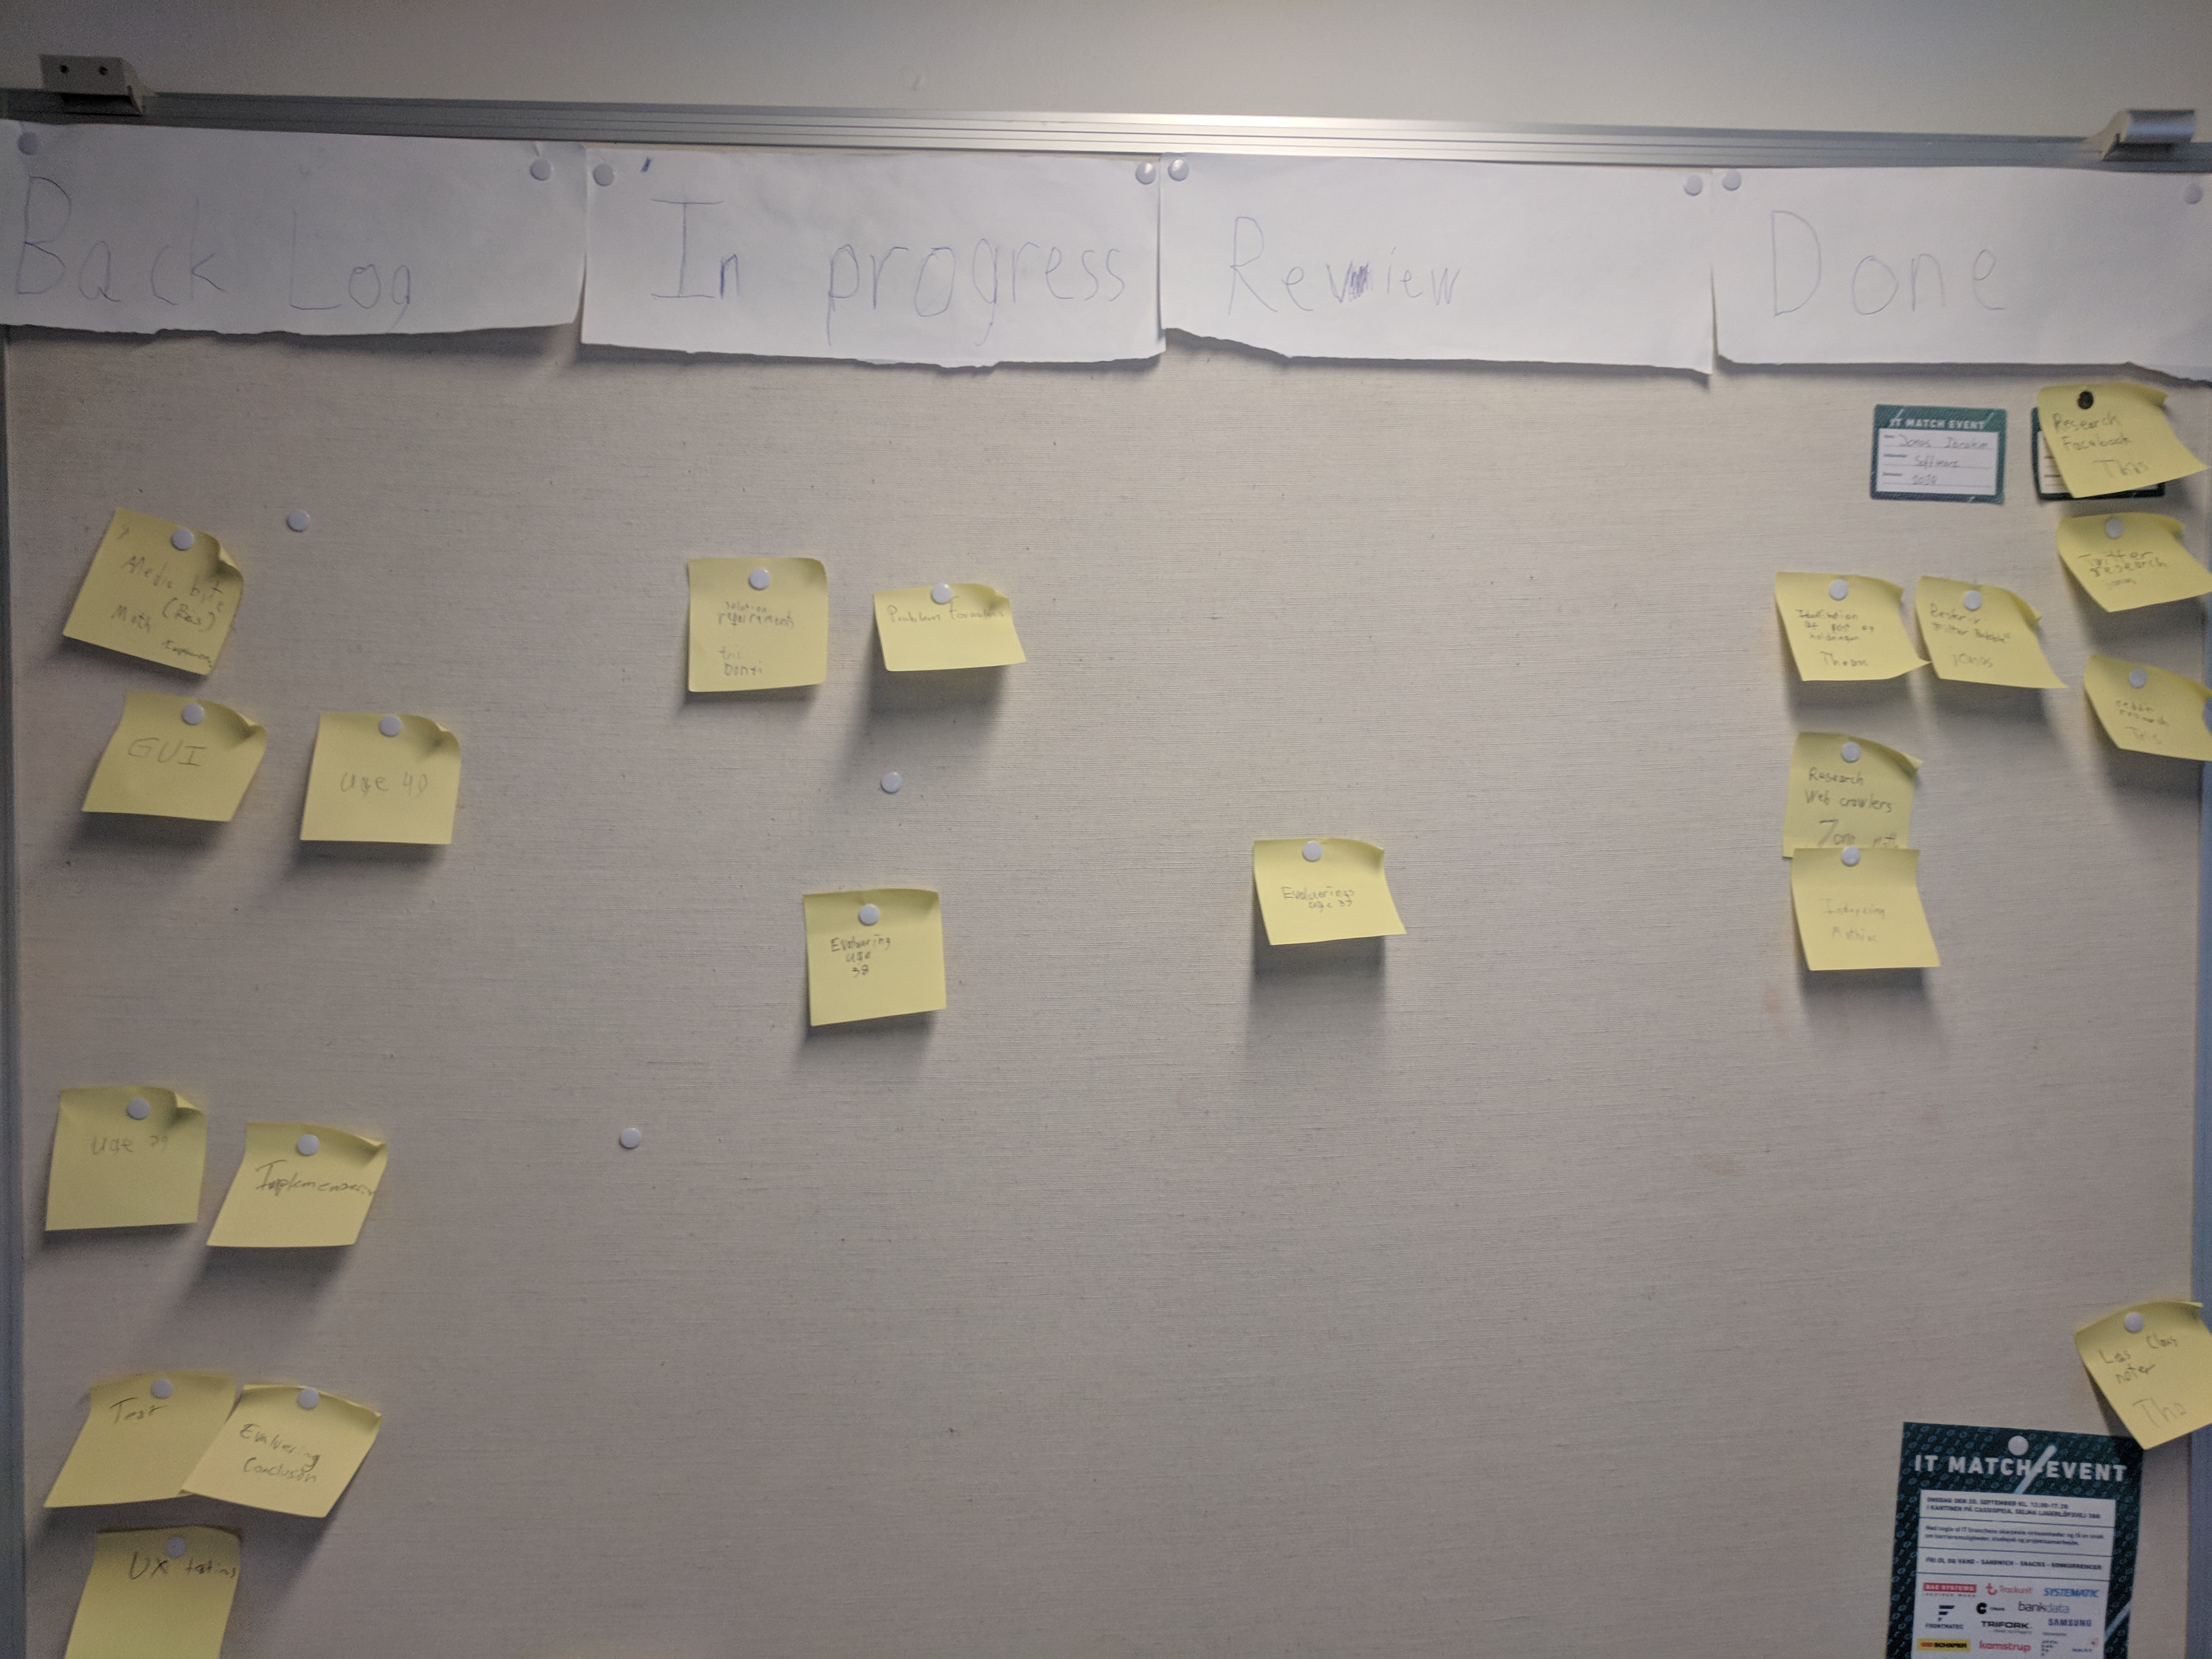
\includegraphics[width = 0.5\textwidth]{figures/Board.jpg}
	\caption{Our board SCRUM element.}
\end{figure}]

\subsection*{Evaluation}
We have investigated further upon what we are able and unable to do with social
media, and further our development on our web crawler. The report is
progressing with some pages in the analysis part as well, the facebook and
filter bubble part is in the editing phase and almost finishedl.
But there is not many gaps in our schedule for project work this semester with
all the lectures lectures.
We have made some plans and furthered the groups structure and workflow.
We made a short description of the final product, but it was mainly for the
suporvisor to see, and will definetly be updated after.
We found that Facebook is very restrictive with its userdata, and does not like
give it away easily. We would have to ask for permission to crawl Facebook and
from the limited amount of crawlers permimtted to do so, then its unlikely that
we get the chance. Therefore we are starting to look further into Twitter and
Reddit as our userdata source, on the initial lookup Twitter's data looks
accessable. 

\subsection*{Next Week}
During the next week we want to finish the parts of the report in editing, and
get the rest of the analysis into the editing phase. We would also like to get
started on the data gahtering part of the report. Nedxt week will have focus on
indexing the sites crawled, which means we hope that we are able to see the data
we will be working with.